% Optional insertion examples; compile from ./final with graphicx loaded.
% These figures describe info's delivered designs. Match the paper's numerical
% results and algorithm description before inserting them into a full paper.

\begin{figure}[htbp]
  \centering
  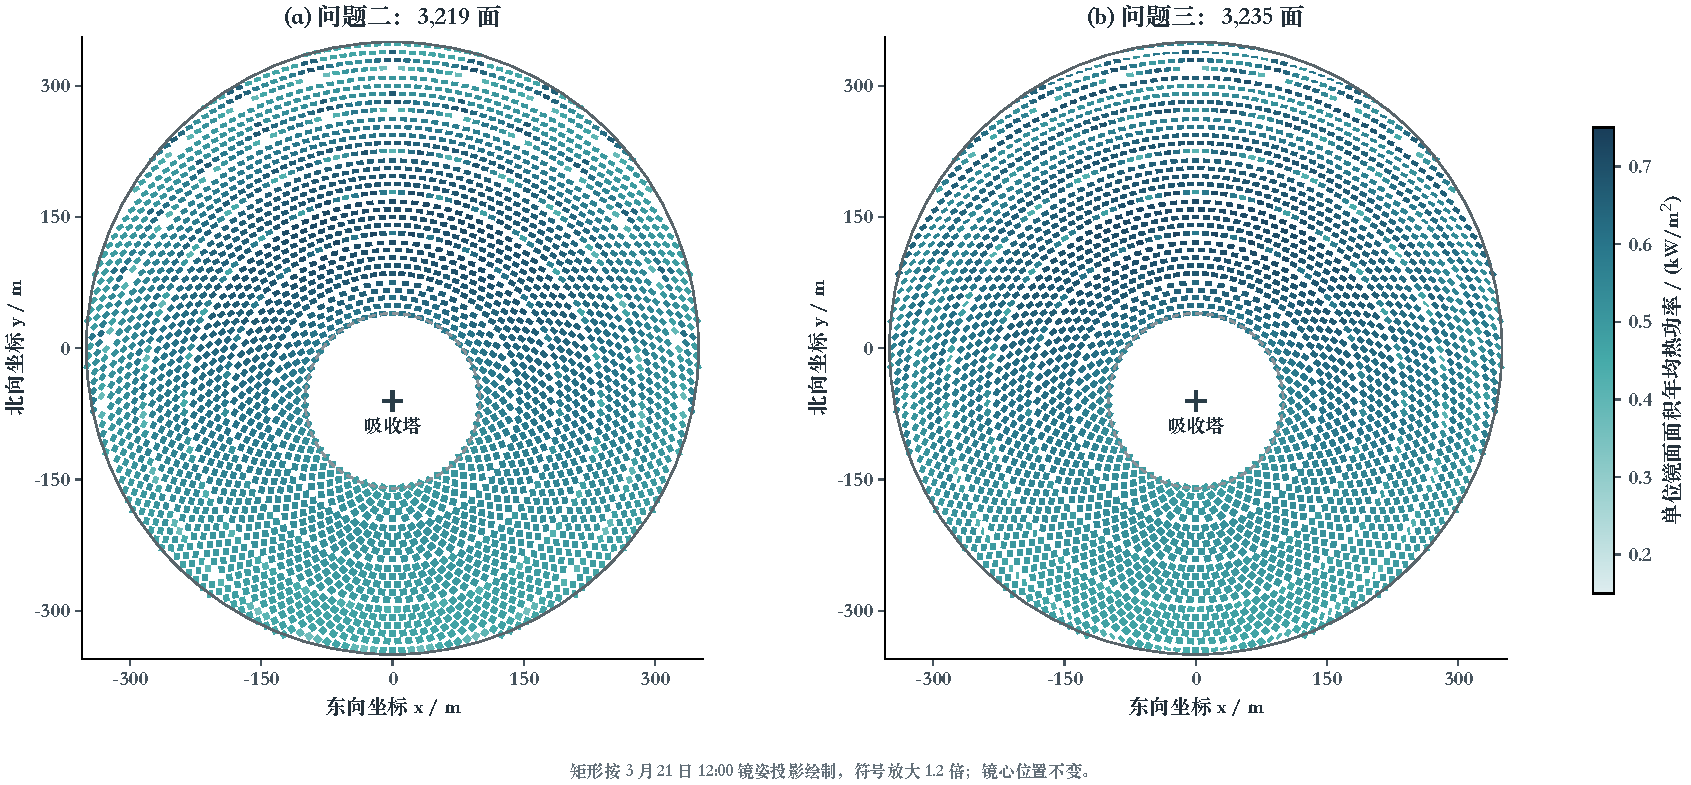
\includegraphics[width=\linewidth]{info_figures/04_q2_q3_comparison.pdf}
  \caption{第二、三问定日镜场布局与单位镜面面积年均热功率。
  实线为半径 $350\,\mathrm{m}$ 的场界，虚线为塔周 $100\,\mathrm{m}$ 禁布区。
  矩形按春分日正午镜姿投影绘制，线性放大 $1.2$ 倍，镜心位置保持原值。}
  \label{fig:info-layout-comparison}
\end{figure}

\begin{figure}[htbp]
  \centering
  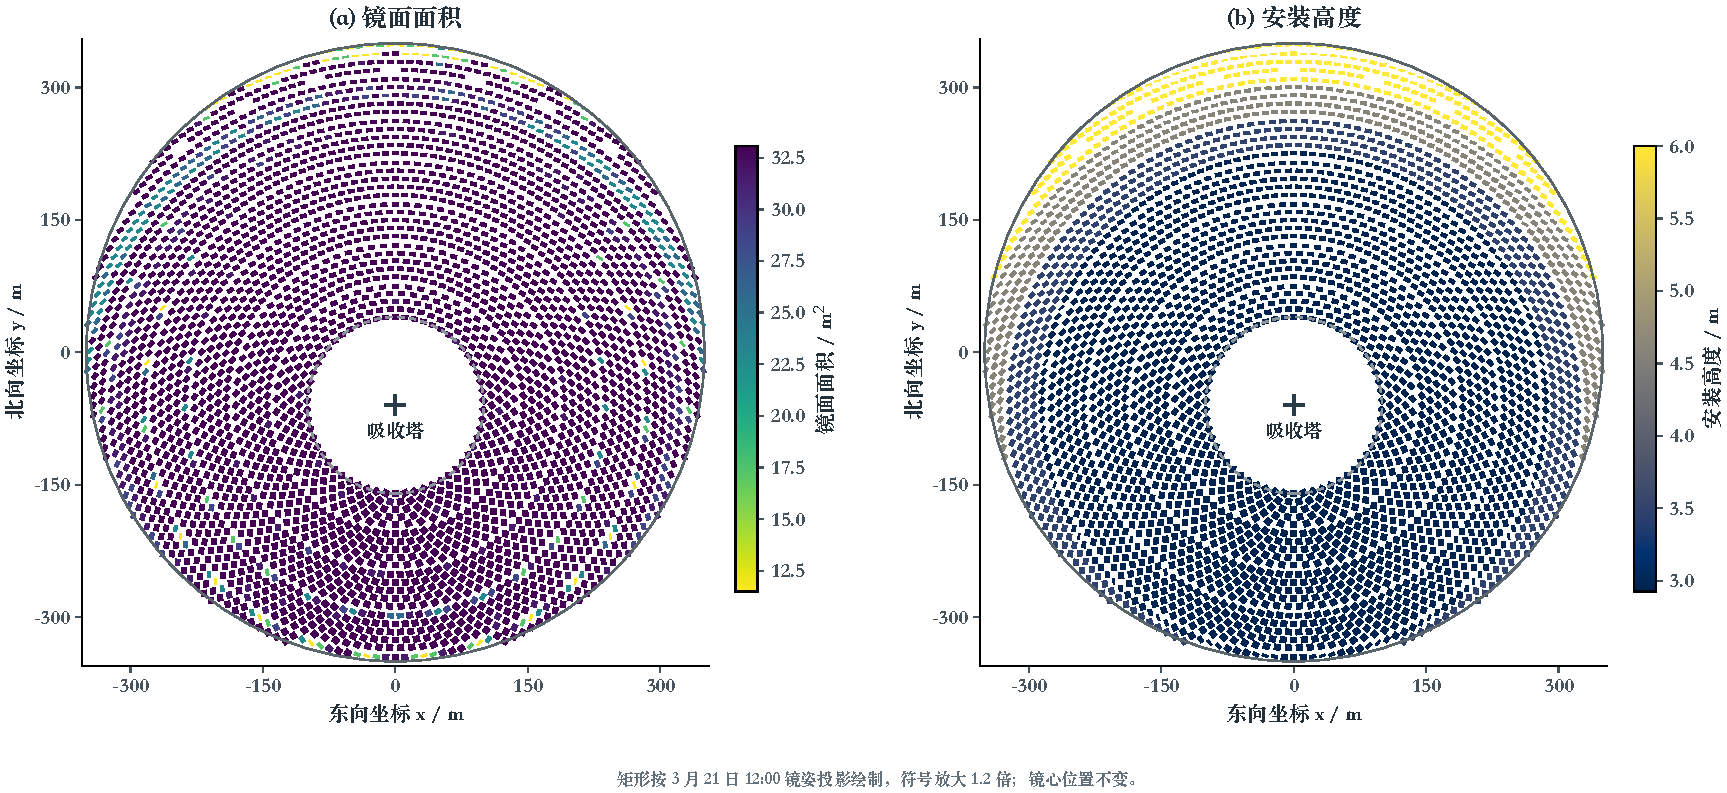
\includegraphics[width=\linewidth]{info_figures/05_q3_area_and_height.pdf}
  \caption{第三问镜面面积与安装高度空间分布。左图颜色表示实际镜面面积，
  右图颜色表示镜面中心安装高度，两图采用相同底座坐标。}
  \label{fig:info-q3-geometry}
\end{figure}

\begin{figure}[htbp]
  \centering
  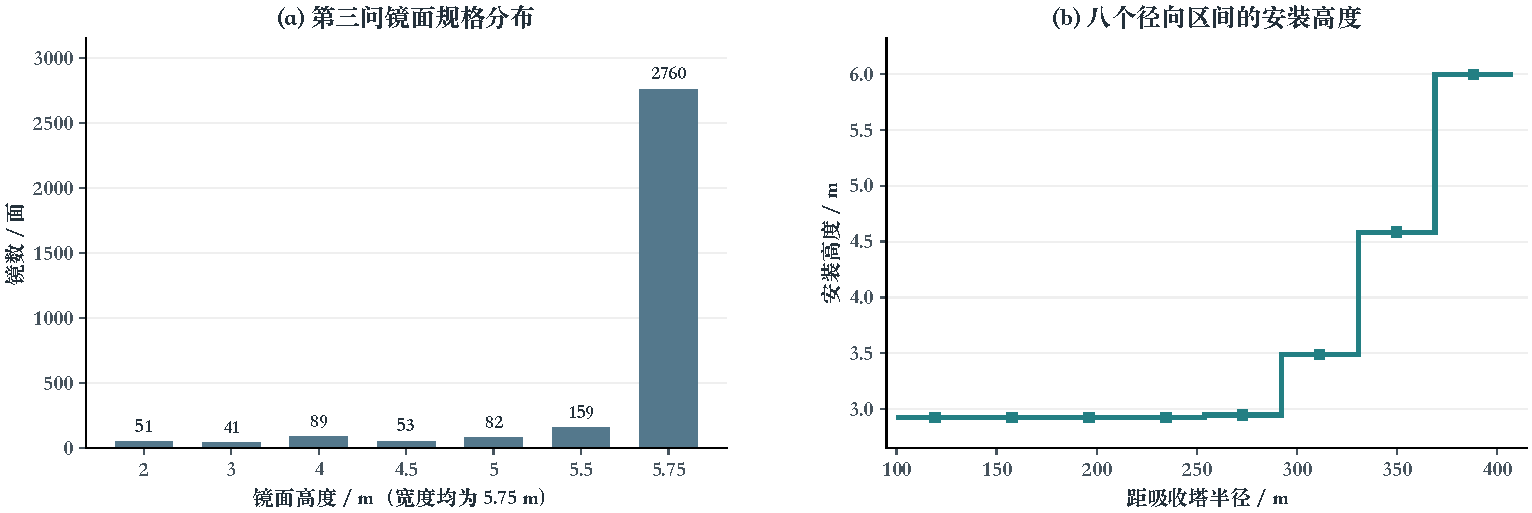
\includegraphics[width=\linewidth]{info_figures/06_q3_specifications.pdf}
  \caption{第三问镜面规格及径向安装高度。镜宽统一为 $5.75\,\mathrm{m}$，
  镜面高度采用七种规格，八个径向区间采用六档安装高度。
  安装高度单调不降及最外层 $6\,\mathrm{m}$ 为算法设定。}
  \label{fig:info-q3-specifications}
\end{figure}

\begin{figure}[htbp]
  \centering
  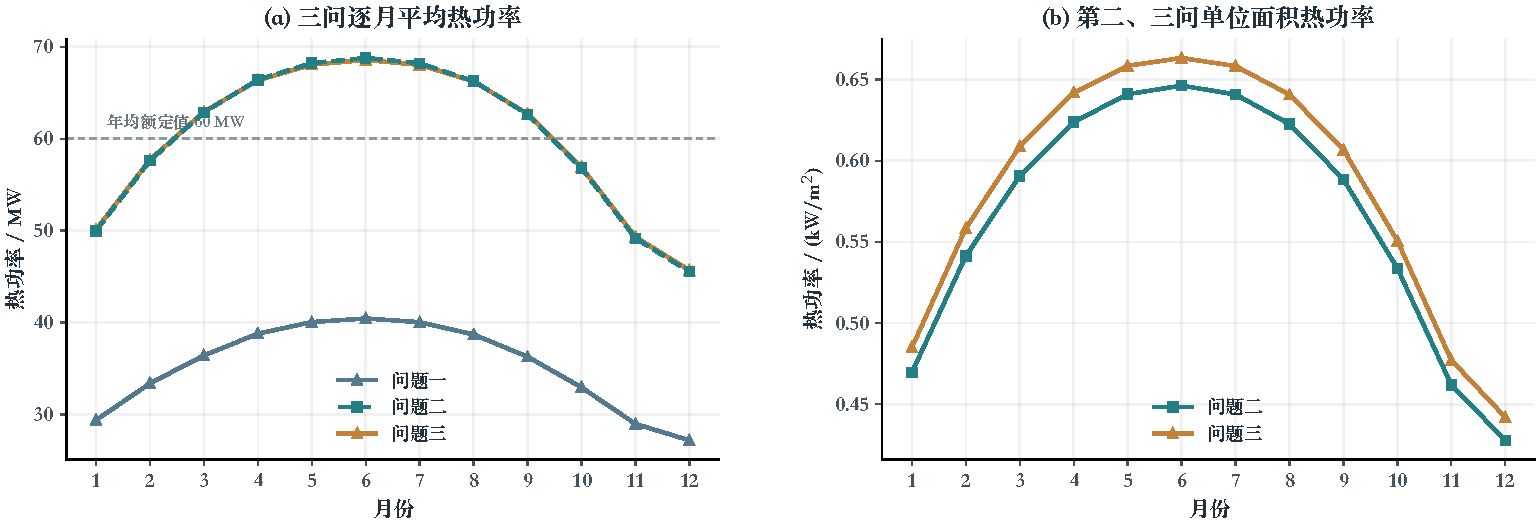
\includegraphics[width=\linewidth]{info_figures/07_monthly_power.pdf}
  \caption{三问月均热功率与第二、三问单位面积热功率。
  每月对 $21$ 日五个规定时刻取平均；$60\,\mathrm{MW}$ 为年均额定要求。}
  \label{fig:info-monthly-power}
\end{figure}

\begin{figure}[htbp]
  \centering
  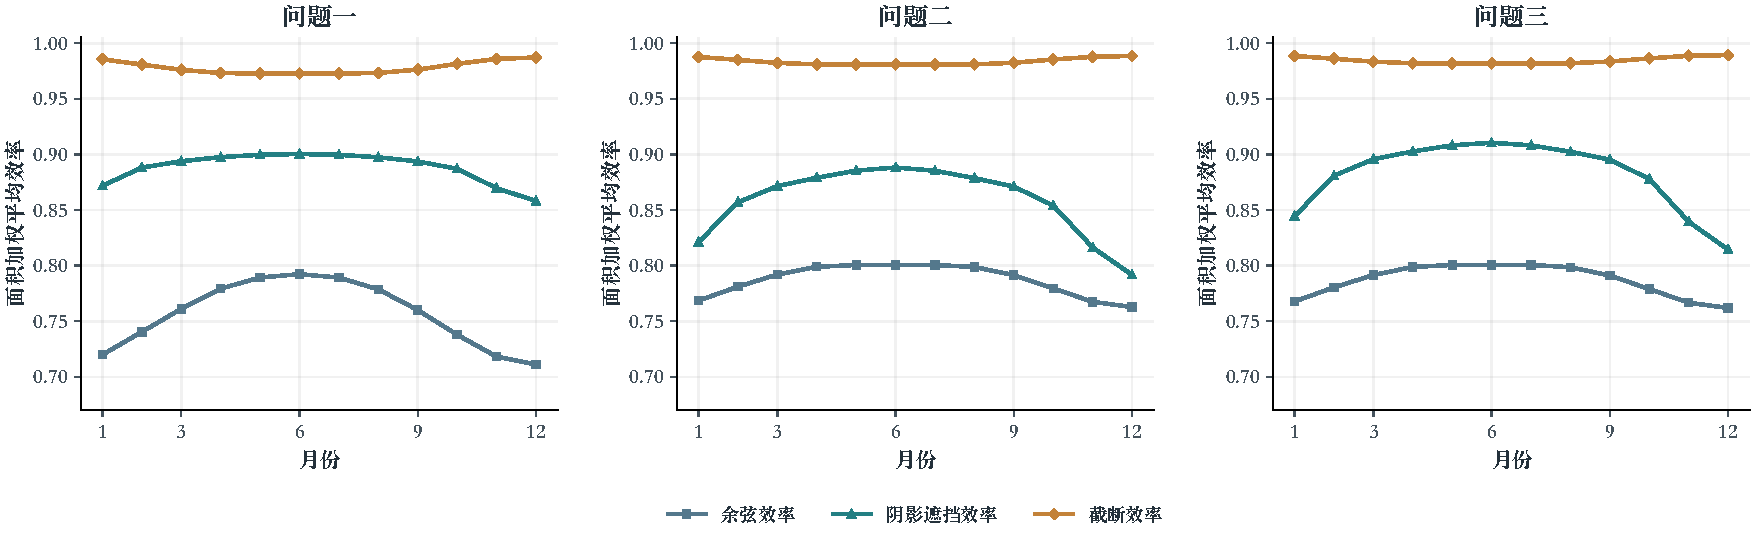
\includegraphics[width=\linewidth]{info_figures/08_monthly_efficiencies.pdf}
  \caption{三问月平均分项效率。各时刻先按镜面面积加权，
  再对当月五个规定时刻取平均。}
  \label{fig:info-monthly-efficiency}
\end{figure}

\begin{figure}[htbp]
  \centering
  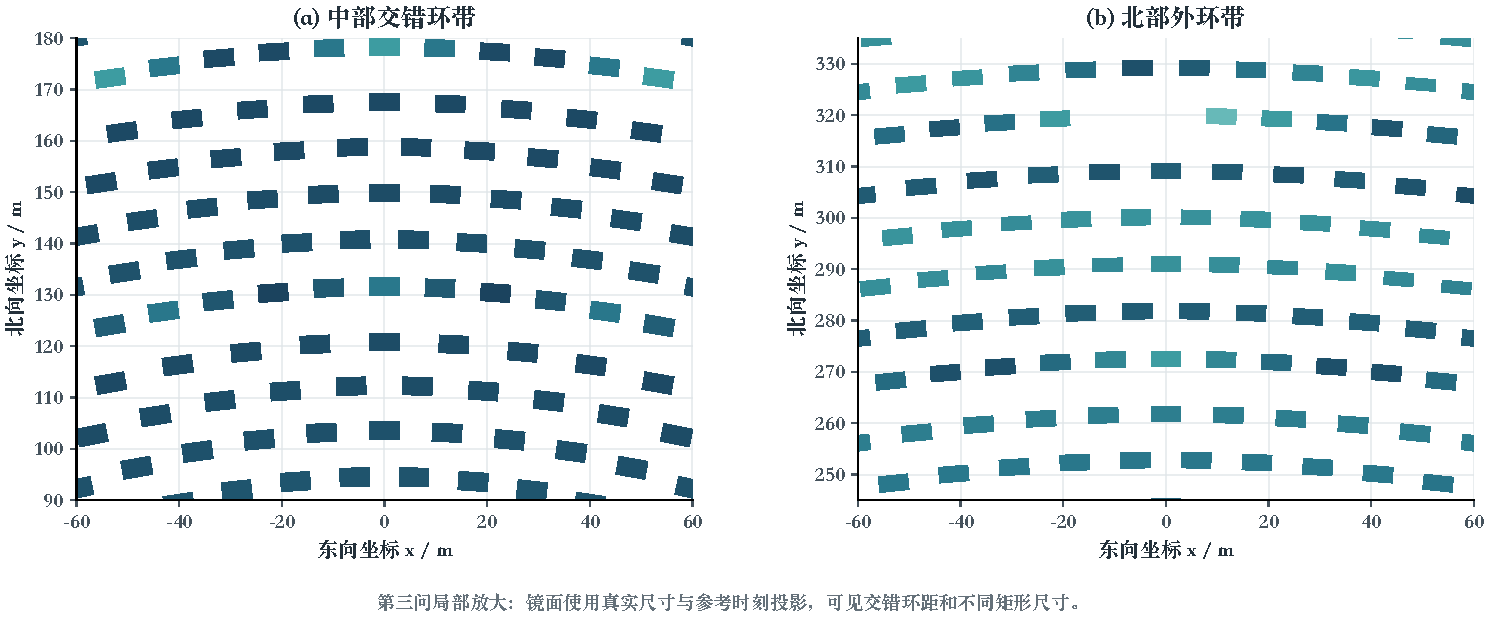
\includegraphics[width=\linewidth]{info_figures/09_q3_rectangle_detail.pdf}
  \caption{第三问中部与北部外环带的局部放大图。
  镜面按真实尺寸在参考时刻的俯视投影等比例绘制。}
  \label{fig:info-mirror-detail}
\end{figure}
